\documentclass[conference,onecolumn]{IEEEtran}
\usepackage{enumitem}
\usepackage{cite}
\usepackage{graphicx}
\usepackage{float}
\graphicspath{{./images}}

\title{XM Radio Reception with the PlutoSDR}

\author{
\IEEEauthorblockN{Owen Sowatzke}
\IEEEauthorblockA{\textit{Electrical Engineering Department} \\
\textit{University of Arizona}\\
Tucson, USA \\
osowatzke@arizona.edu}
\and
\IEEEauthorblockN{Glenn Alan Walker}
\IEEEauthorblockA{\textit{Electrical Engineering Department} \\
\textit{University of Arizona}\\
Tucson, USA \\
gaw@arizona.edu}}

\begin{document}
\maketitle

XM radio leverages a combination of satellites and terrestrial repeaters to diversify its transmitted signal. The satellites transmit QSPK-modulated symbols, and the terrestrial repeaters leverage COFDM modulation \cite{5586866}. For our final project, we propose demodulating the signal from a single satellite and performing forward error correction (FEC). Our project will leverage the time, frequency, and frame synchronization methods covered in class. Additionally, it will extend the material covered in class to forward error correction. XM radio is a proprietary signal, and the technical details are documented only in patents such as \cite{a2008_us8260192b2, marko_2012_us8667344b2}. Major milestones for our project include: performing timing and frequency synchronization, extracting the master frame preamble (MFP) and frame synchronization preamble (FSP), and demodulating the signal from a single satellite. Additional stretch goals that will be addressed only if time permits include: demodulating the COFDM signals from terrestrial repeaters, combining the returns from multiple satellites and/or the terrestrial repeaters, and playing XM channel 1 audio (free preview channel). We believe that this project will reinforce what we learned in the course and provide invaluable experience performing FEC and OFDM demodulation.

\iffalse
\begin{figure}[H]
	\centerline{\fbox{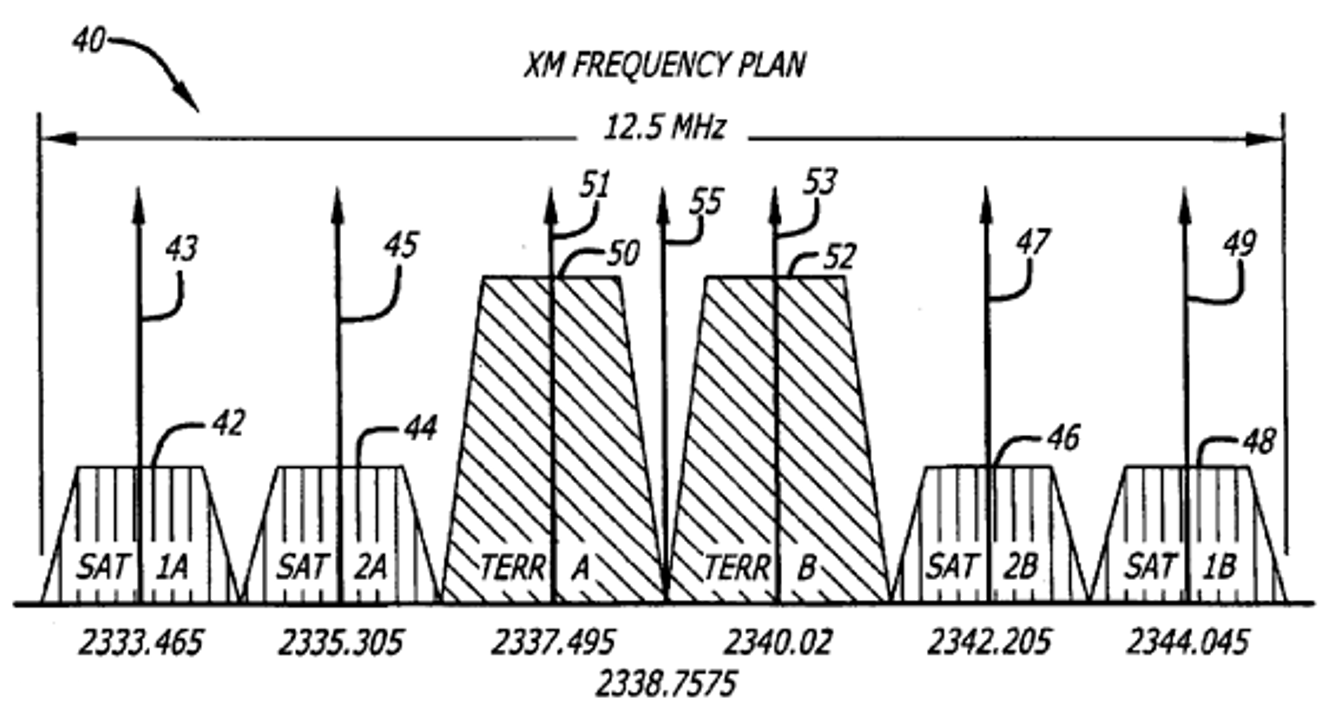
\includegraphics[width=0.5\textwidth]{xm_spectrum.png}}}
	\caption{XM Radio Spectrum \cite{a1999_us6724827b1}}
	\label{fig::xm_spectrum}
\end{figure}
\fi

\begin{figure}[H]
	\centerline{\fbox{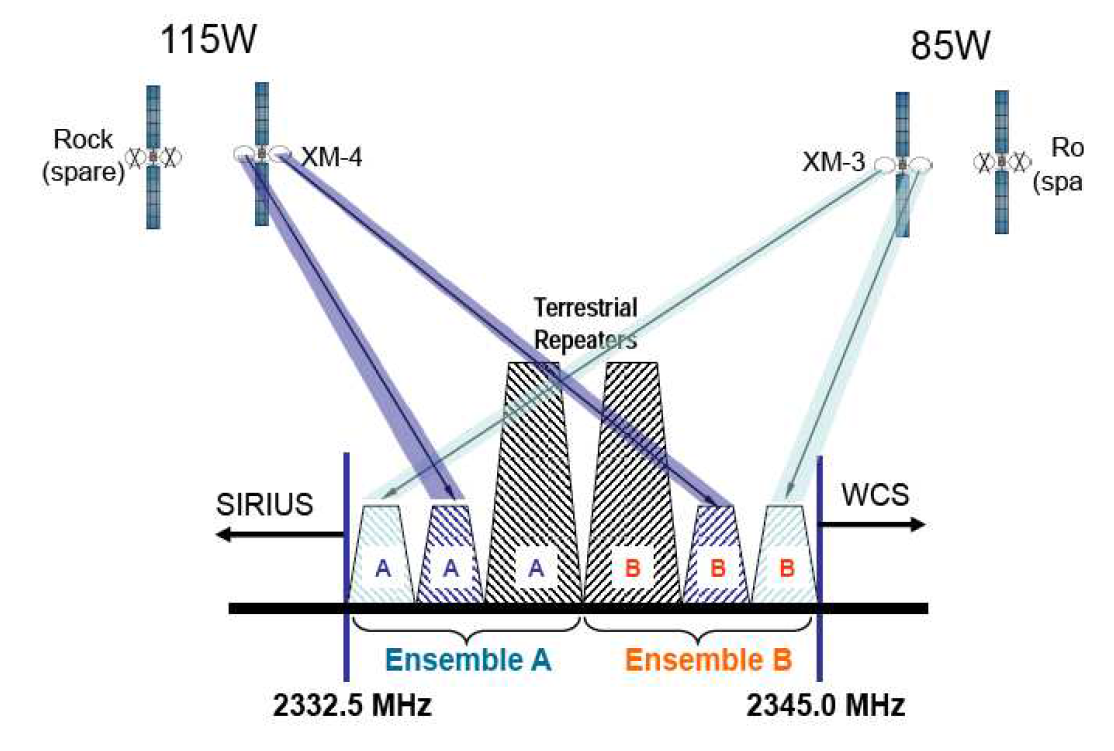
\includegraphics[width=0.5\textwidth]{xm_satellite_config.png}}}
	\caption{XM Radio Satellite Configuration \cite{5586866}}
	\label{fig::xm_satellite_config}
\end{figure}

XM Radio divides their content across two separate ensembles (Ensemble A and Ensemble B), which are illustrated in Figure \ref{fig::xm_satellite_config}. Each ensemble uses transmitter diversity to improve signal quality and prevent dropouts. The diversity scheme specifically uses QPSK-modulated signals from two separate satellites and a terrestrial COFDM-modulated signal. We concentrate specifically on the TDM receiver. An example of its architecture is displayed in Figure \ref{fig::tdm_receiver}. 

\begin{figure}[H]
	\centerline{\fbox{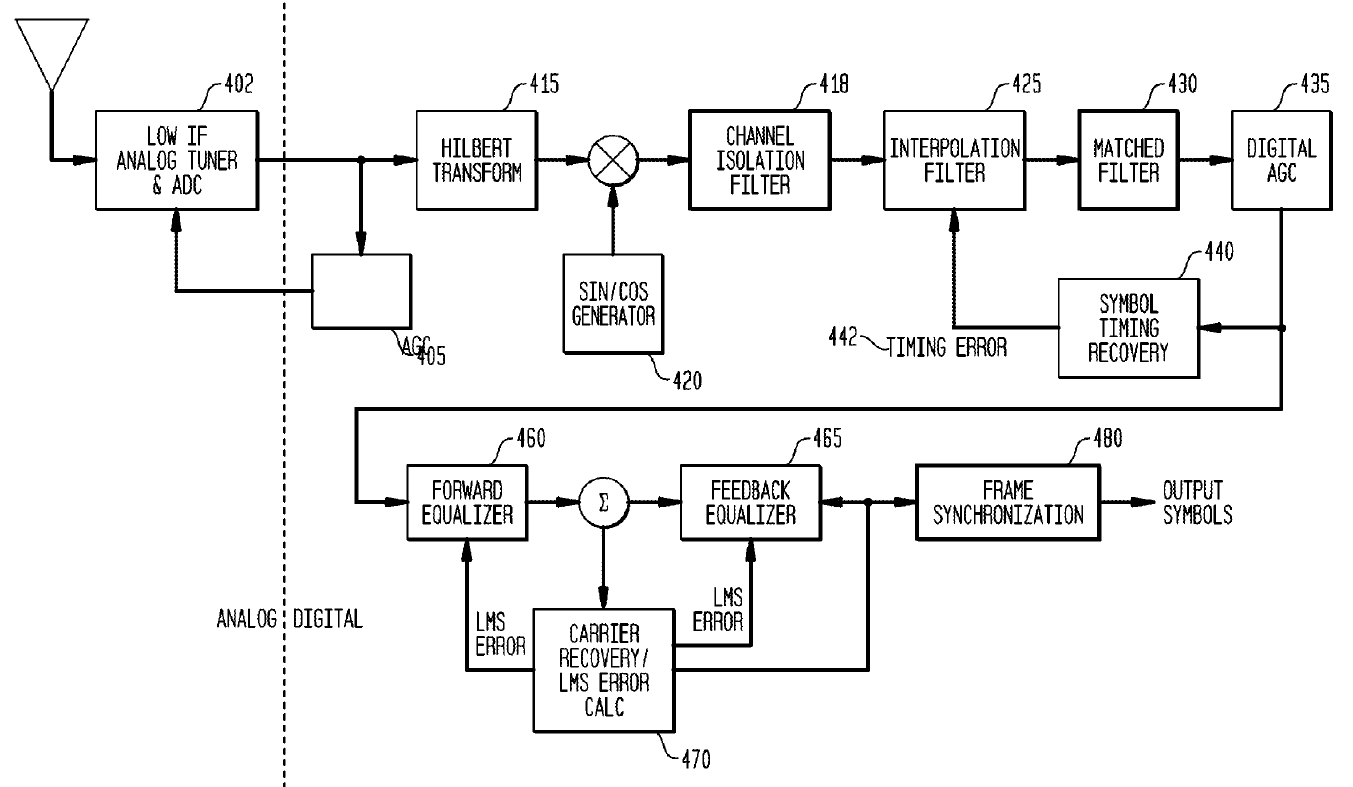
\includegraphics[width=0.5\textwidth]{tdm_receiver.png}}}
	\caption{TDM Receiver Architecture \cite{a2008_us8260192b2}}
	\label{fig::tdm_receiver}
\end{figure}


\begin{figure}[H]
	\centerline{\fbox{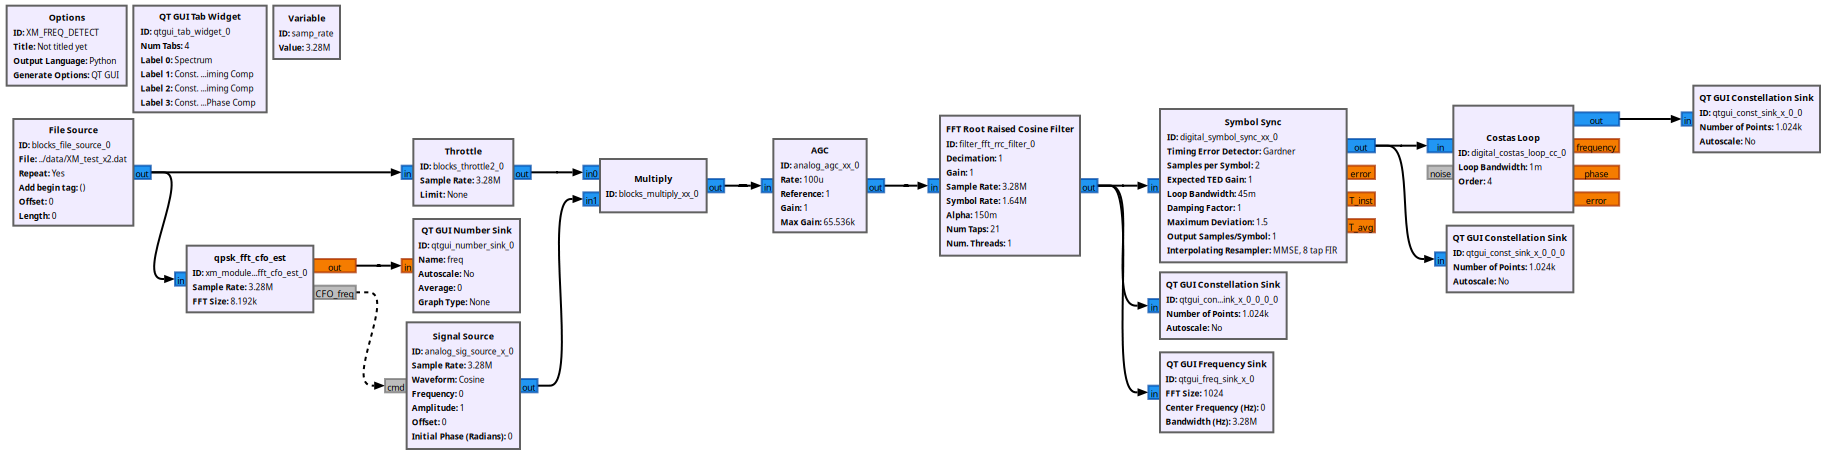
\includegraphics[width=0.8\textwidth]{timing_carrier_sync.png}}}
	\caption{GNU Radio Flowchart That Implements Timing and Carrier Synchronization}
	\label{fig::timing_carrier_sync}
\end{figure}

\begin{itemize}
	\item Nyquist Filter
	\item Timing Synchronization
	\item Carrier Compensation
	\begin{itemize}
		\item Coarse
		\item Fine
	\end{itemize}
	\item Frame Synchronization
\end{itemize}

\nocite{5586866}
\nocite{a2008_us8260192b2}
\nocite{marko_2012_us8667344b2}
\nocite{collins_2018_softwaredefined}
\nocite{chaudhari_2022_timing}
\nocite{650240}
\bibliographystyle{IEEEtran}
\bibliography{sources}{}
%\bibliographystyle{ieeetr}
\end{document}